\documentclass{article}
\usepackage[utf8]{inputenc}

\title{Economic Impact of COVID 19 Under a Consumer Spending and Business Revenue Perspective}
\author{Rui Xin, Tony Wu, George Wang, Zeyu Shen}
\date{November 2020}

\usepackage[margin=1.0in]{geometry}
\usepackage{enumitem}
\usepackage{amsmath}
\usepackage{amssymb}
\usepackage{graphicx}
\usepackage{enumitem}
\usepackage[english]{babel}
\usepackage{amsthm}
\usepackage{comment}
\usepackage{float}
\usepackage{tikz}
\usepackage[ruled,vlined]{algorithm2e}
\begin{document}

\maketitle

\section{Abstract}
We present a methodology for studying the economic impact of COVID-19 on cities under a consumer spending and business revenue perspective. We find in one year, places like Chicago will be most severely affected by COVID-19, followed by Los Angeles, while Charlotte is the least affected one among the cities we investigate. In general, we concluded that cities with lots of small industries and decreased population mobility are most severely affected.

\section{Introduction}
COVID-19 is dramatically changing the world, both socially and economically. Many cities are flustering under the pandemic, while some are not so much affected. In this paper, we present a methodology for studying the economic impact of COVID-19 on cities under a consumer spending and business revenue perspective. In particular, we focus on how COVID-19 impact domestic cities and do not take cities outside America into account.
\par
As the single most important indicator for economic activities, GDP consists of consumer spending, government expenditure, imports and exports and business revenue. Among them, we will assume that government expenditure is uniform across most cities, which makes sense because even if differences do exist, its influence would be overshadowed by changes in the other three parts. Also, we do not investigate the influence of imports and exports as we focus our attention on domestic situations. Consumer spending and business revenue will be the protagonist of our analysis, as they are closely related to the well-being of cities. 
\par
In this paper, we first choose economic factors (covariates) that are possibly correlated with consumer spending and business revenue. Then, we run a dimensionality reduction process with Gibbs sampling to remove uncorrelated or loosely correlated covariates. Furthermore, we conduct time series forecast for the remaining economic factors in selected regions. Ultimately, we train a model with neural network, providing the predictions for the covariates as input, and obtain predictions for how much cities will be affected in the following year, which will also shed light on which type of cities would be most acutely influenced.

\section{Choice of Covariates and Dimensionality Reduction}
Consumer spending and business revenue depend on a lot of economic factors, and it's hard to directly predict their trends in the future. Therefore, we will consider them as dependent variables and choose a number of independent variables that are easier to apply time series forecast on, and then establish relationship between them.
\par
In particular, we propose the following possible covariates, or independent variables: change in rate of employment for low-income, middle-income, and high-income workers, respectively, income level, population, the cumulative number of cases, the number of new cases and population mobility. In total, there are eight covariates. We split the change in the rate of employment into three covariates because the rate of change varies significantly for these three types of workers. 
\par
Then, we run a dimensionality reduction process with Gibbs sampling using continuous spike prior. In particular, we use student t-distribution as prior because it provides heavier tails and thus more similar to a dirac spike prior, which is typically used for variable selection. The result gives that the cumulative number of COVID cases, income level, and population have little predictive value for change in consumer spending, while population and income level has little predictive value for change in business revenue. Thus, we will not take population and income value into account in the following sections and focus our attention on the remaining six covariates. 


\section{Time Series Forecast for Economic Factors in Selected Regions}
\par
To illustrate the economic impacts of COVID-19 across different regions in the United States, we select Los Angeles (CA), Chicago (IL), and Charlotte (NC) and perform time series forecast on their rates of employment across income levels and their residents' mobility, both of which are crucial independent variables indicating their respective economic status. These three cities are chosen because they are scattered broadly across the US and thus represent vastly different types of cities and because their data of employment rate changes and are have been sufficiently collected. The data we use for our time series forecast is collected from Opportunity Insight's EconomicTracker dataset, which span from early January to late October and could be considered as up-to-date.  

\par
To predict these economic factors for the near future, we choose the ARIMA model. The ARIMA combines autoregression and moving average and is often shown to be effective in time series prediction tasks. Previous researches have employed ARIMA for COVID-19 cases forecast \cite{tandon2020coronavirus}, and some even found that ARIMA outperformed some deep learning models despite the latter's increasing popularity in industry in recent years \cite{papastefanopoulos2020covid}. Considering that the economic factors we investigate are directly related to the trend of COVID cases, we believe that ARIMA could also be effective in forecasting the employment rate changes and mobility changes induced by the pandemic. Specifically, we set the value of each variable in January as benchmark and predict the percentage of change compared to their respective benchmark. Our forecast results (red part of the curve in the following figures) of the employment rates by income levels and time spent at home are as followed: 


\begin{figure}[ht]
\begin{minipage}[b]{0.3\linewidth}
\centering
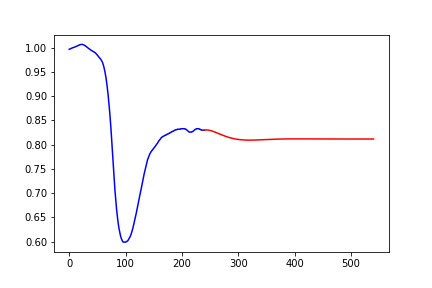
\includegraphics[width=\textwidth]{Charlotte_lowinc_emp.png}
\caption{Charlotte, low income}
\end{minipage}
\hspace{0.5cm}
\begin{minipage}[b]{0.3\linewidth}
\centering
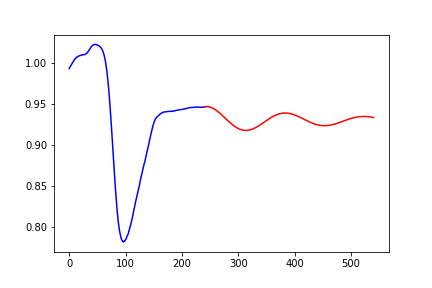
\includegraphics[width=\textwidth]{Charlotte_midinc_emp.png}
\caption{Charlotte, mid income}
\end{minipage}
\hspace{0.5cm}
\begin{minipage}[b]{0.3\linewidth}
\centering
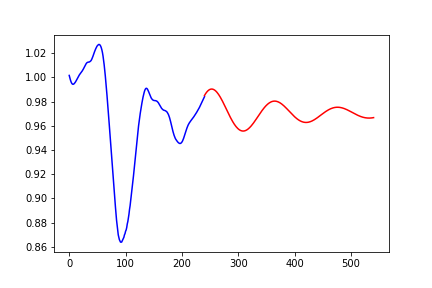
\includegraphics[width=\textwidth]{Charlotte_highinc_emp.png}
\caption{Charlotte, high income}
\end{minipage}
\end{figure}

\begin{figure}[ht]
\begin{minipage}[b]{0.3\linewidth}
\centering
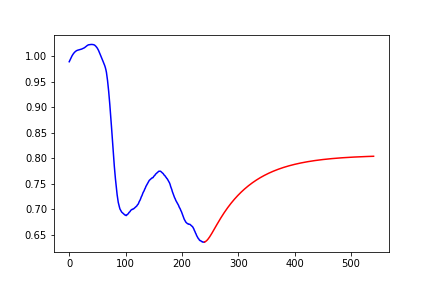
\includegraphics[width=\textwidth]{Chicago_lowinc_emp.png}
\caption{Chicago, low income}
\end{minipage}
\hspace{0.5cm}
\begin{minipage}[b]{0.3\linewidth}
\centering
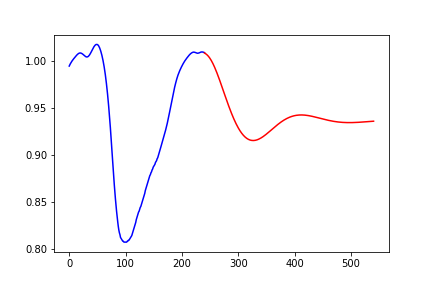
\includegraphics[width=\textwidth]{Chicago_midinc_emp.png}
\caption{Chicago, mid income}
\end{minipage}
\hspace{0.5cm}
\begin{minipage}[b]{0.3\linewidth}
\centering
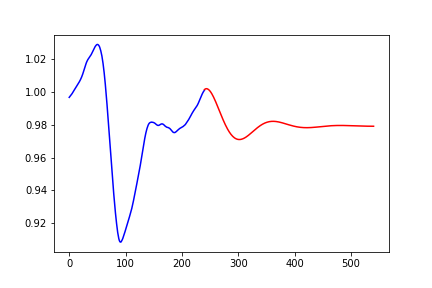
\includegraphics[width=\textwidth]{Chicago_highinc_emp.png}
\caption{Chicago, high income}
\end{minipage}
\end{figure}

\begin{figure}[ht]
\begin{minipage}[b]{0.3\linewidth}
\centering
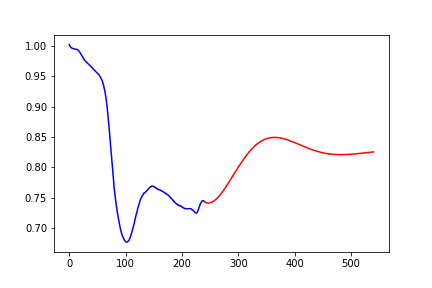
\includegraphics[width=\textwidth]{LA_lowinc_emp.png}
\caption{LA, low income}
\end{minipage}
\hspace{0.5cm}
\begin{minipage}[b]{0.3\linewidth}
\centering
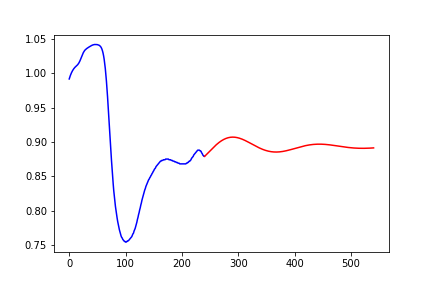
\includegraphics[width=\textwidth]{LA_midinc_emp.png}
\caption{Charlotte, mid income}
\end{minipage}
\hspace{0.5cm}
\begin{minipage}[b]{0.3\linewidth}
\centering
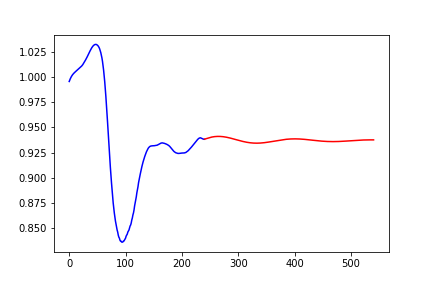
\includegraphics[width=\textwidth]{LA_highinc_emp.png}
\caption{LA, high income}
\end{minipage}
\end{figure}

\begin{figure}[ht]
\begin{minipage}[b]{0.3\linewidth}
\centering
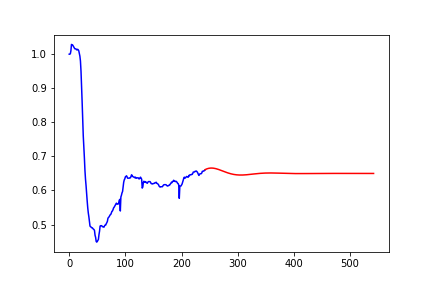
\includegraphics[width=\textwidth]{Charlotte_time_at_workplace.png}
\caption{Charlotte, time spent at workplace}
\end{minipage}
\hspace{0.5cm}
\begin{minipage}[b]{0.3\linewidth}
\centering
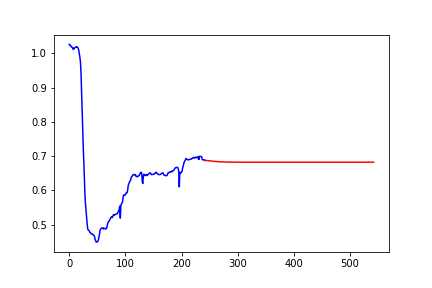
\includegraphics[width=\textwidth]{Chicago_time_at_workplace.png}
\caption{Chicago, time spent at workplace}
\end{minipage}
\hspace{0.5cm}
\begin{minipage}[b]{0.3\linewidth}
\centering
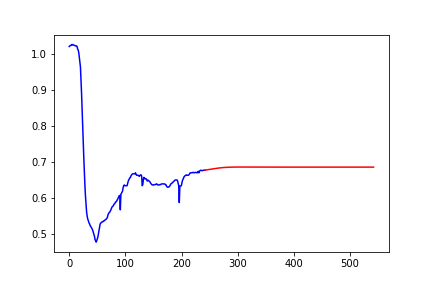
\includegraphics[width=\textwidth]{LA_time_at_workplace.png}
\caption{LA, time spent at workplace}
\end{minipage}
\end{figure}

\section{Model Training and Prediction}
We predict the economic impact of COVID on cities using a sequential neural network architecture with eight inputs and two hidden layers. We implement this model to evaluate and predict the consumer spending and business revenue sectors of the economy. After performing dimensionality reduction and other preliminary data analysis, we picked the following variables as input to the neural network: daily COVID case increase, cumulative COVID cases, average income, employment for low-income workers, employment for medium income workers, employment for high income workers, total population, and mobility factor. We constructed for each label a model based on the input. We can observe the loss decreasing over the epoch over time. With a revised model, we are able to observe the model's predictions being consistent as the result of time series analysis.

\begin{figure}[!htb]
\begin{minipage}[b]{0.49\linewidth}
\centering
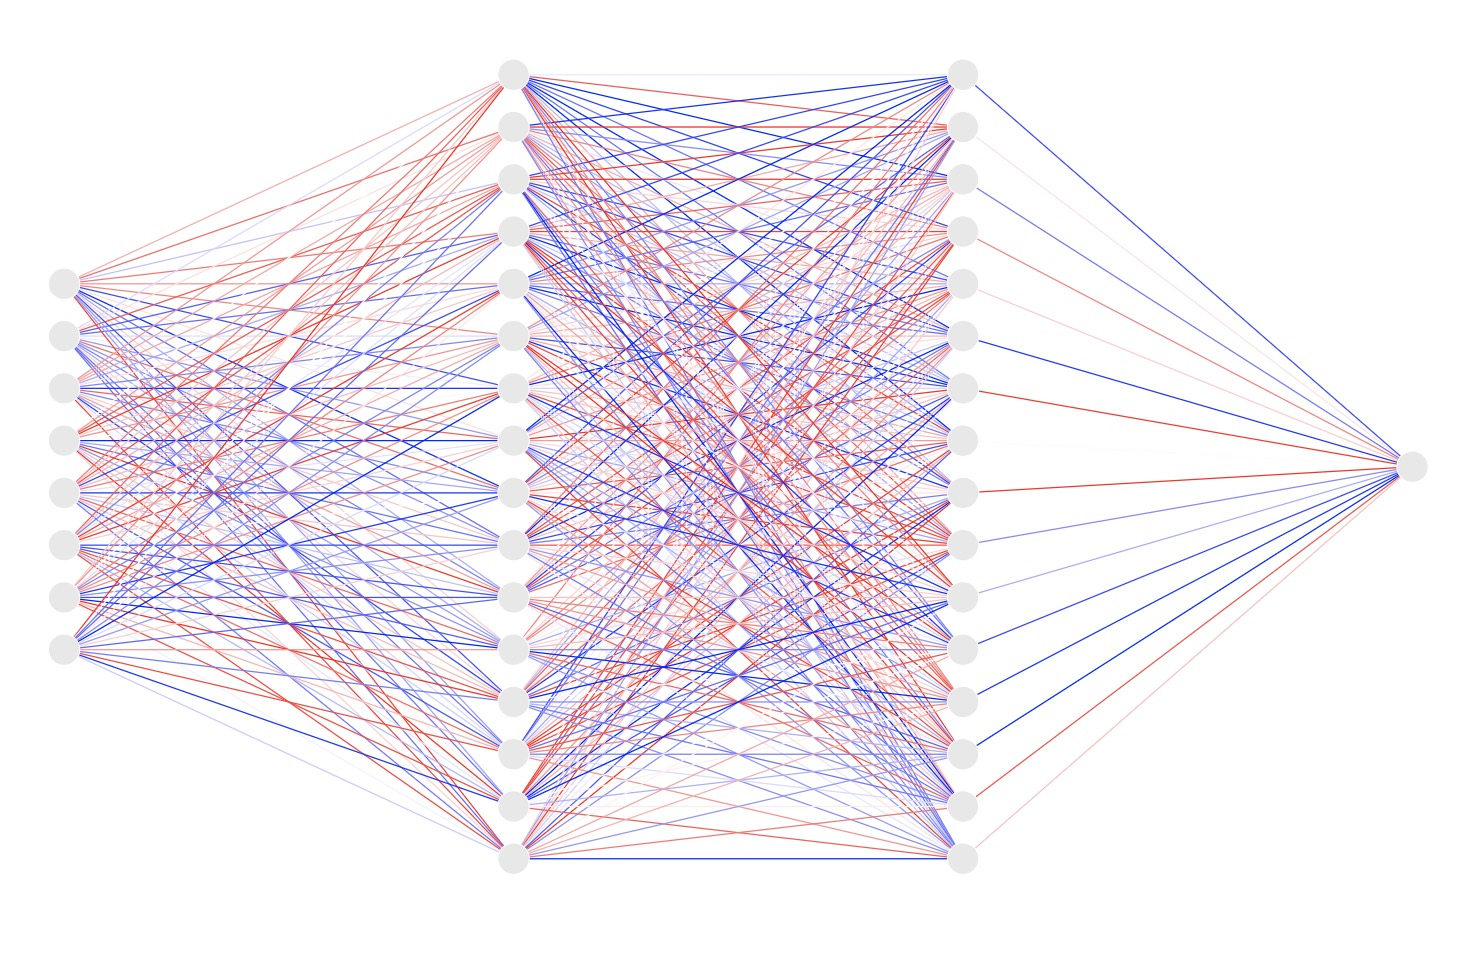
\includegraphics[width=\textwidth]{arch.jpg}
\caption{Network Architecture}
\end{minipage}
\begin{minipage}[b]{0.49\linewidth}
\centering
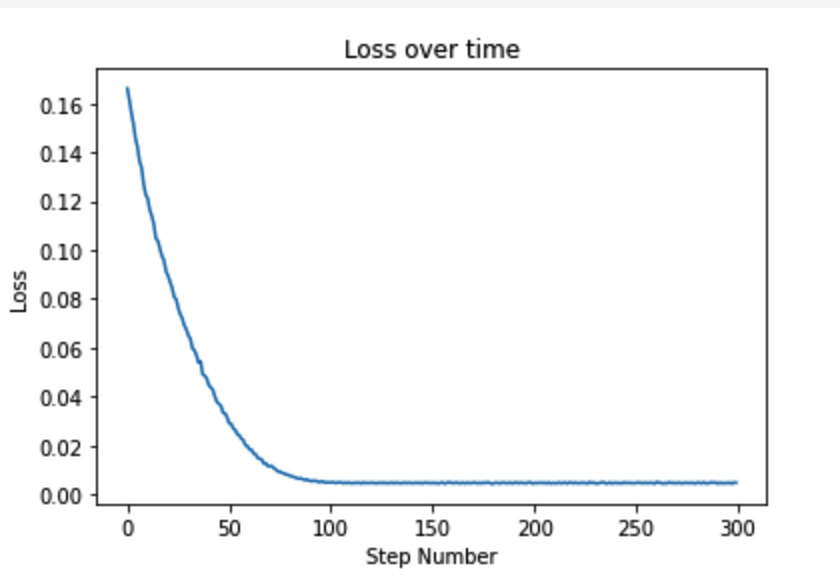
\includegraphics[width=\textwidth, trim={0 0 0 0.5cm},clip]{loss_over_time.png}
\caption{Loss Function Over Time}
\end{minipage}
\end{figure}

\section{Conclusion}
According to our prediction, in one year, Chicago will be most severely affected by COVID-19, Los Angeles follows, while Charlotte is the least affected one. This makes economic sense, as Chicago has the greatest number of small businesses, and many of their lockdowns would lead to high unemployment rate. Moreover, Chicago imposes strict social distancing rules, and social mobility would therefore be impaired as people are forced to stay at homes. Both of these are crucial covariates for predicting consumer spending and business revenue. Los Angeles would also be somewhat affected because it has lots of small businesses, though not as many as Chicago, and social distancing rules. Significant decrease in import and export would also lead to its economic depression. Charlotte would righteously be the least affected one by the similar line of reasoning. In two or five years, there would be much higher uncertainty in prediction, but we can reasonably believe that cities like Chicago with lots of small businesses and strict social distancing rules would still be the most impacted ones, since compared to other industries or agriculture, small businesses are much harder to recover from an economic trough. Closure of deprecation of many small businesses would be irreversible, and its influence can extend to a much wider span of time.

\par
Our model is far from comprehensive, as there are still many possible covariates to consider, such as import, export, or travelling, which would all potentially impose great impact on a city's economy. We also realize that COVID response policies played a vital role in the dynamics of the pandemic, and future economic trends inevitably will depend on new policies. However, our model still demystifies which cities are potentially most affected. In short, our model and analysis predicts that cities with high number of small businesses and decreased mobility, or away-from-home rate, are likely to suffer the most. These impacts could last more than 1 year, and perhaps up to 5 years, because the short-term changes of economic factors such as decreased employment rate are related to more long-lasting effects, such as bankruptcy of small businesses and even larger chain stores. According to our findings, cities should promptly take actions to tackle unemployment, such as offering short-term job opportunities (projects similar to president Roosevelt's New Deal could be potential options), before its economic situation exacerbate even more severely. Moreover, since the amount of time residents spend at workplace has shown significant amount of decrease and is likely to persist for a period of time, cities can also consider innovative ways to offer more remote jobs to boost the economy.

\newpage

\bibliographystyle{acm}
\bibliography{citation}
\end{document}
